%--------------------------------------------------------------------
%--------------------------------------------------------------------
% Formato para los talleres del curso de Métodos Computacionales
% Universidad de los Andes
% 2015, curso de vacaciones
%--------------------------------------------------------------------
%--------------------------------------------------------------------

\documentclass[11pt,legalpaper]{exam}
\usepackage[utf8]{inputenc}
\usepackage[spanish]{babel}
\usepackage{graphicx}
\usepackage{mdframed}
\usepackage{tabularx}
\usepackage[absolute]{textpos} % Para poner una imagen en posiciones arbitrarias
\usepackage{multirow}
\mdfdefinestyle{mystyle}{leftmargin=1cm,rightmargin=1cm,linecolor=red}
\usepackage{float}
\usepackage{hyperref}
\decimalpoint

\newcommand{\base}[1]{\underline{\hspace{#1}}}
\boxedpoints
\pointname{ pt}
%\extrawidth{0.75in}
%\extrafootheight{-0.5in}
\extraheadheight{-0.15in}
\hypersetup{%
  colorlinks=true,% hyperlinks will be coloured
  urlcolor=blue
}

%\noprintanswers
%\printanswers
\renewcommand{\solutiontitle}{}
\SolutionEmphasis{\color{blue}}

\usepackage{upquote,textcomp}
\newcommand\upquote[1]{\textquotesingle#1\textquotesingle} % To fix straight quotes in verbatim
\newcommand{\ihat}{\,\hat{\textbf{\i}}}
\newcommand{\jhat}{\,\hat{\textbf{\j}}}

\begin{document}
\begin{center}
{\Large Métodos Computacionales} \\
Tarea 6 - \textsc{Cálculo Simbólico \& PDE } \\
Julio de 2015
\end{center}

\begin{textblock*}{40mm}(10mm,20mm)
  
\includegraphics[width=3cm]{logoUniandes.png}
\end{textblock*}

\begin{textblock*}{40mm}(164mm,20mm)
  
\includegraphics[width=3cm]{logoUniandes.png}
\end{textblock*}

\vspace{0.5cm}

La solución a esta tarea debe cargarse a su repositorio en GitHub en la carpeta /MC/Tareas/HW6/ como un  cuaderno de nombre \verb+HW6.ipynb+. En el cuaderno dedicar una sección a cada ejercicio con subsecciones para cada literal. Es requisito que en todo lo hecho se pongan comentarios que expliquen lo que se está haciendo.  

La fecha límite de entrega es el \textbf{viernes 10 de julio a las 23:59}. Puede trabajarse en parejas.

\vspace{0.5cm}

\begin{questions}
 
\question[40] \textbf{Cálculo Simbólico} \\[0.5cm]
 En este ejercicio queremos usar \verb+Sympy+ para calcular las ecuaciones que definen a los métodos explícitos de Adams-Bashforth para cualquier orden.
\begin{parts}
	\part[20] Programe una función de \verb+python+ llamada \verb+lagrange+ que reciba el número N de puntos $\left\{ t_i, f_i \right\}$ para  $i=0...,N-1$, y que entregue de regreso una expresión simbólica para el polinomio de grado $N-1$ que los interpola. Puede usar \href{http://docs.sympy.org/dev/modules/core.html?highlight=var#sympy.core.symbol.var}{var} para definir símbolos de \verb+SymPy+ de forma programática y \href{http://docs.sympy.org/dev/modules/core.html?highlight=var#sympy.core.symbol.var}{eval} para convertir strings en nombres de objetos. Abajo a la izquierda se muestra el output en algunos casos.\\[0.1cm]

\begin{center}
	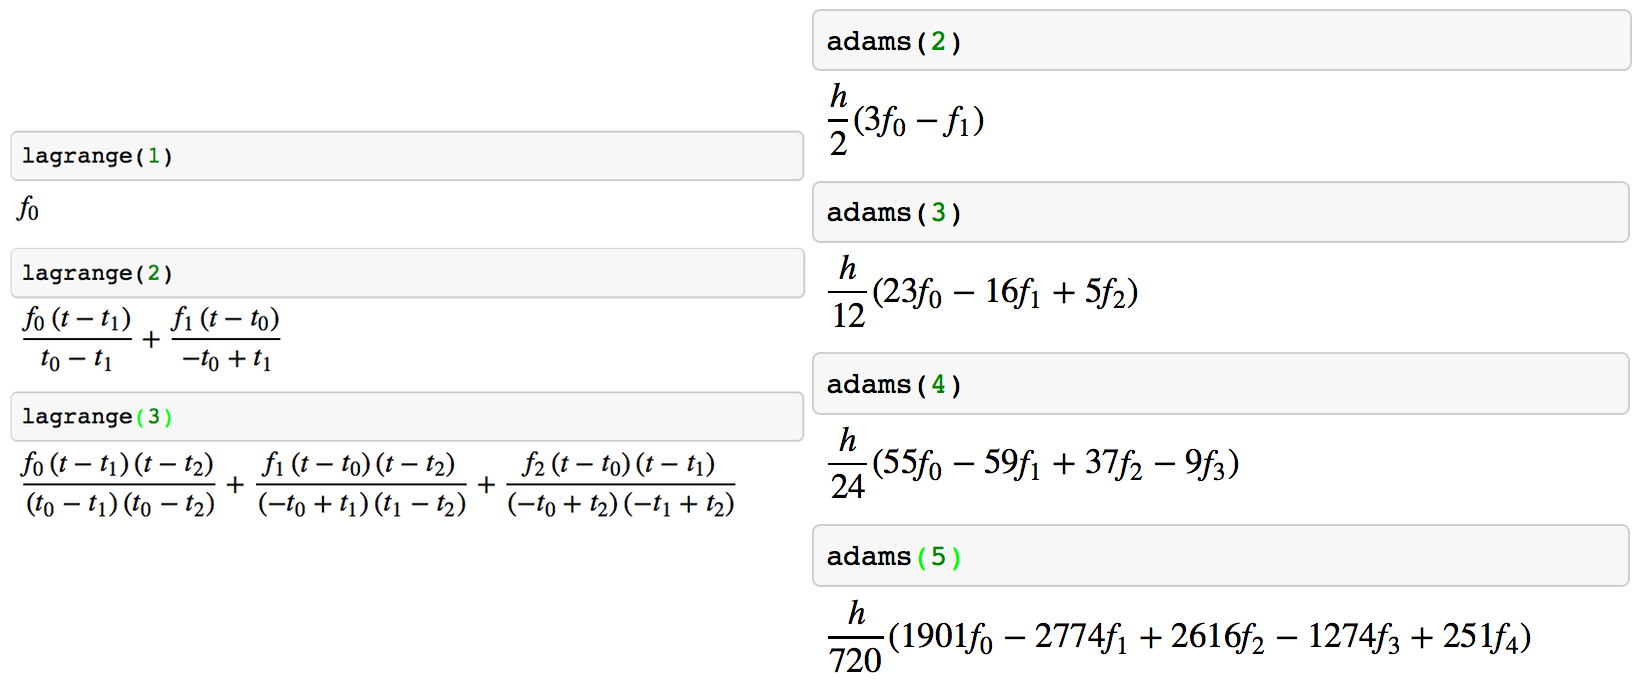
\includegraphics[width=0.95\textwidth]{./adamsandlagrange.png}
\end{center}

	\part[20] Ahora, en el contexto de los métodos {\it multistep} de Adams-Bashforth defina una función llamada \verb+adams+ que reciba el orden $m$ a considerar y de regreso entregue el incremento correspondiente. Para ello tome $t_i = t_n - i*h$ y $f_i = f(t_i)$ siendo $h$ el {\it timestep}. Para ello debe utilizar la función definida en el anterior literal, y utilizar \verb+integrate+ y \verb+simplify+ de \verb+SymPy+. Arriba a la derecha se muestra el output en algunos casos.\\[0.1cm]
	
\begin{center}
	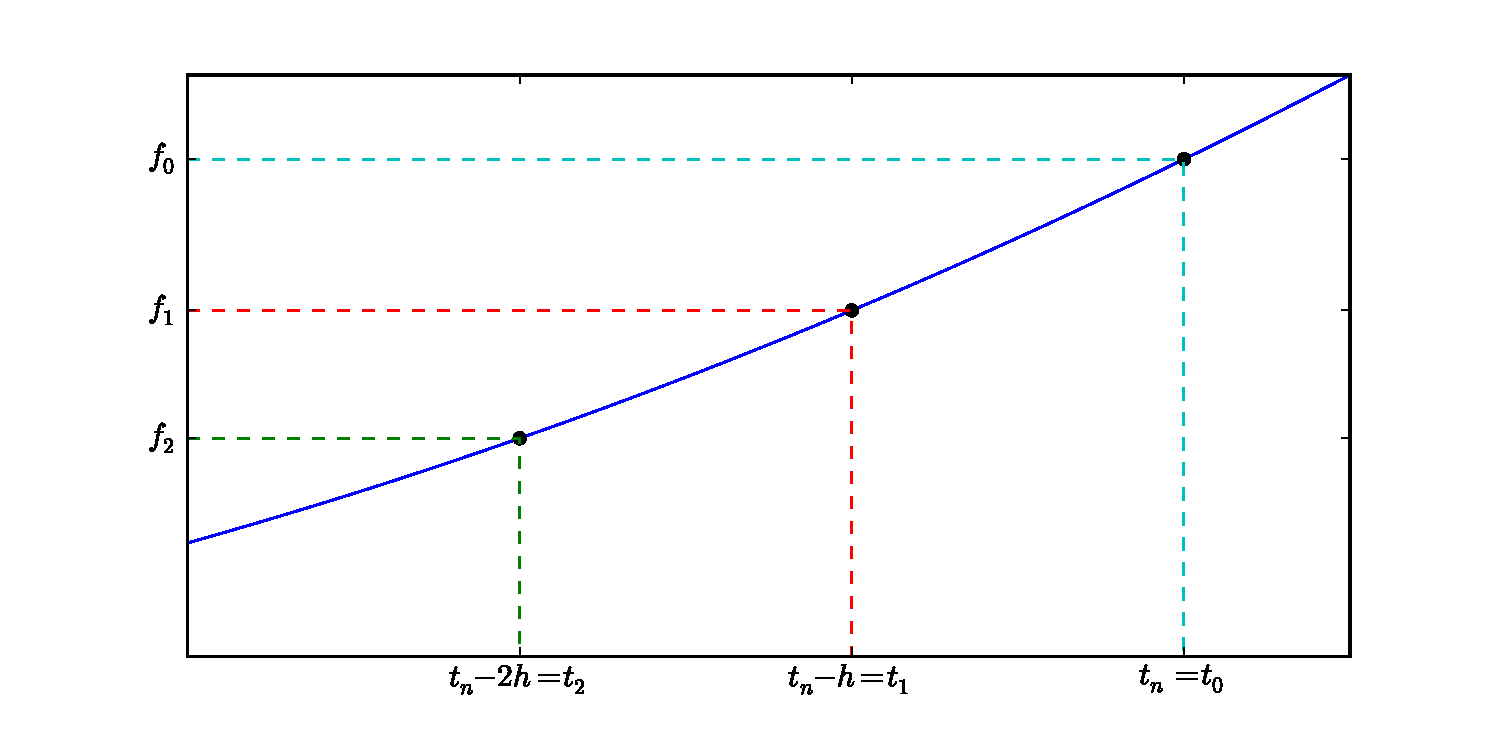
\includegraphics[width=0.95\textwidth]{adam_plot.pdf}
\end{center}
	
\end{parts}

\newpage

\question[60] En este ejercicio queremos encontrar la solución a la ecuación de Poisson para el caso del potencial gravitacional y usar el resultado para resolver la ecuación de movimiento de una pequeña partícula. Para poder hacerlo debe modificar lo visto para la ecuación de Poisson en el caso electromagnético para el caso gravitacional.

\begin{parts}
\part[20]
Encuentre el potencial gravitacional de un cubo de densidad $400.\frac{\textrm{g}}{\textrm{cm}^3}$ y lado $270.\,\textrm{m}$ usando el método de relajación. Resuelva la ecuación de Poisson para el potencial en un cubo de $3.00\,\textrm{km}$ de lado usando una cuadrícula en cada dirección de $30.\,\textrm{m}$ de lado. Use condiciones de frontera de Dirichlet tomando $\phi=0$ en la frontera y tome como {\it ansatz} el potencial de una masa puntual. Use un sistema de coordenadas con el centro del cubo en el origen y los ejes $xyz$ perpendiculares a las caras. Al final haga una gráfica de densidad del potencial en el plano $yz$ con líneas equipotenciales superpuestas. 

\begin{center}
	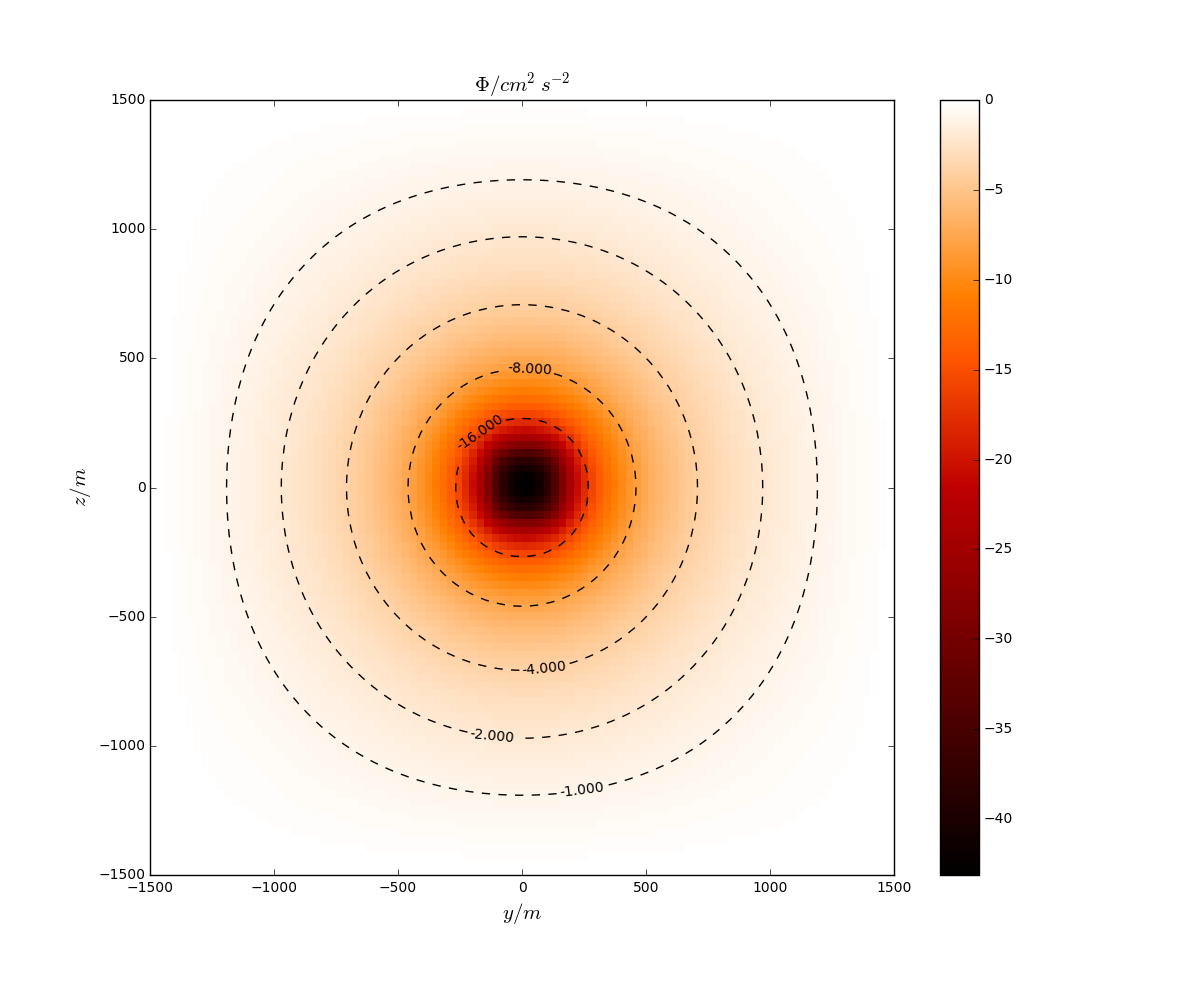
\includegraphics[width=0.85\textwidth]{./yzpotential.png}
\end{center}

\part[15]
También haga una gráfica del potencial a lo largo del eje $z$ y compare con lo que se obtiene de segmentar el cubo en $9^3$ masas puntuales y sumar los potenciales correspondientes.

\begin{center}
	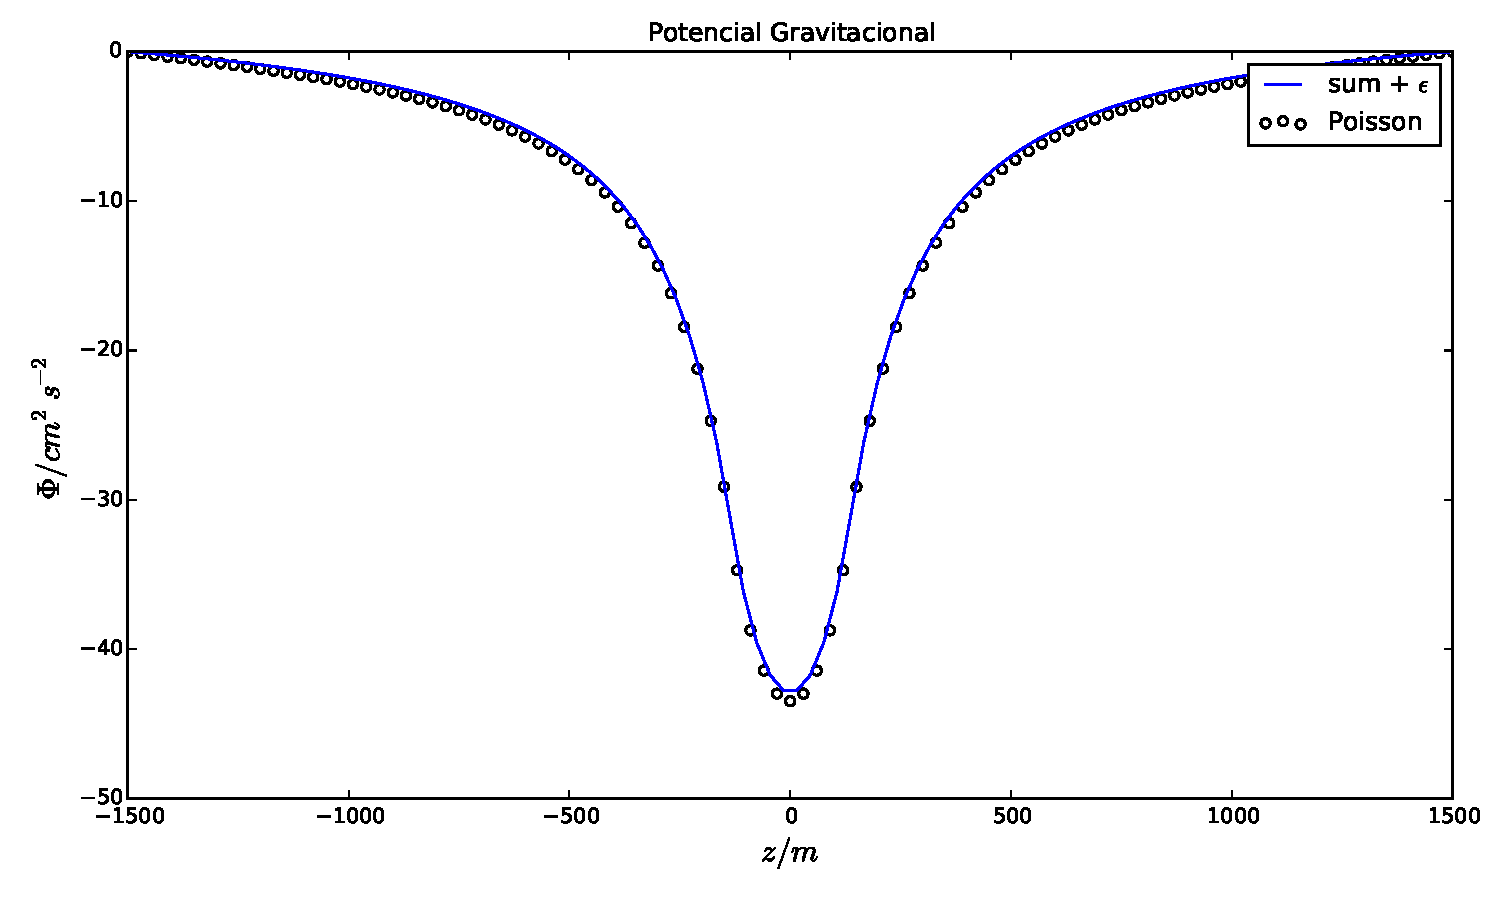
\includegraphics[width=0.85\textwidth]{./zpotential.pdf}
\end{center}
\newpage
\part[15] Luego calcule el campo gravitacional a lo largo del mismo eje haciendo derivadas numéricas. 

\begin{center}
	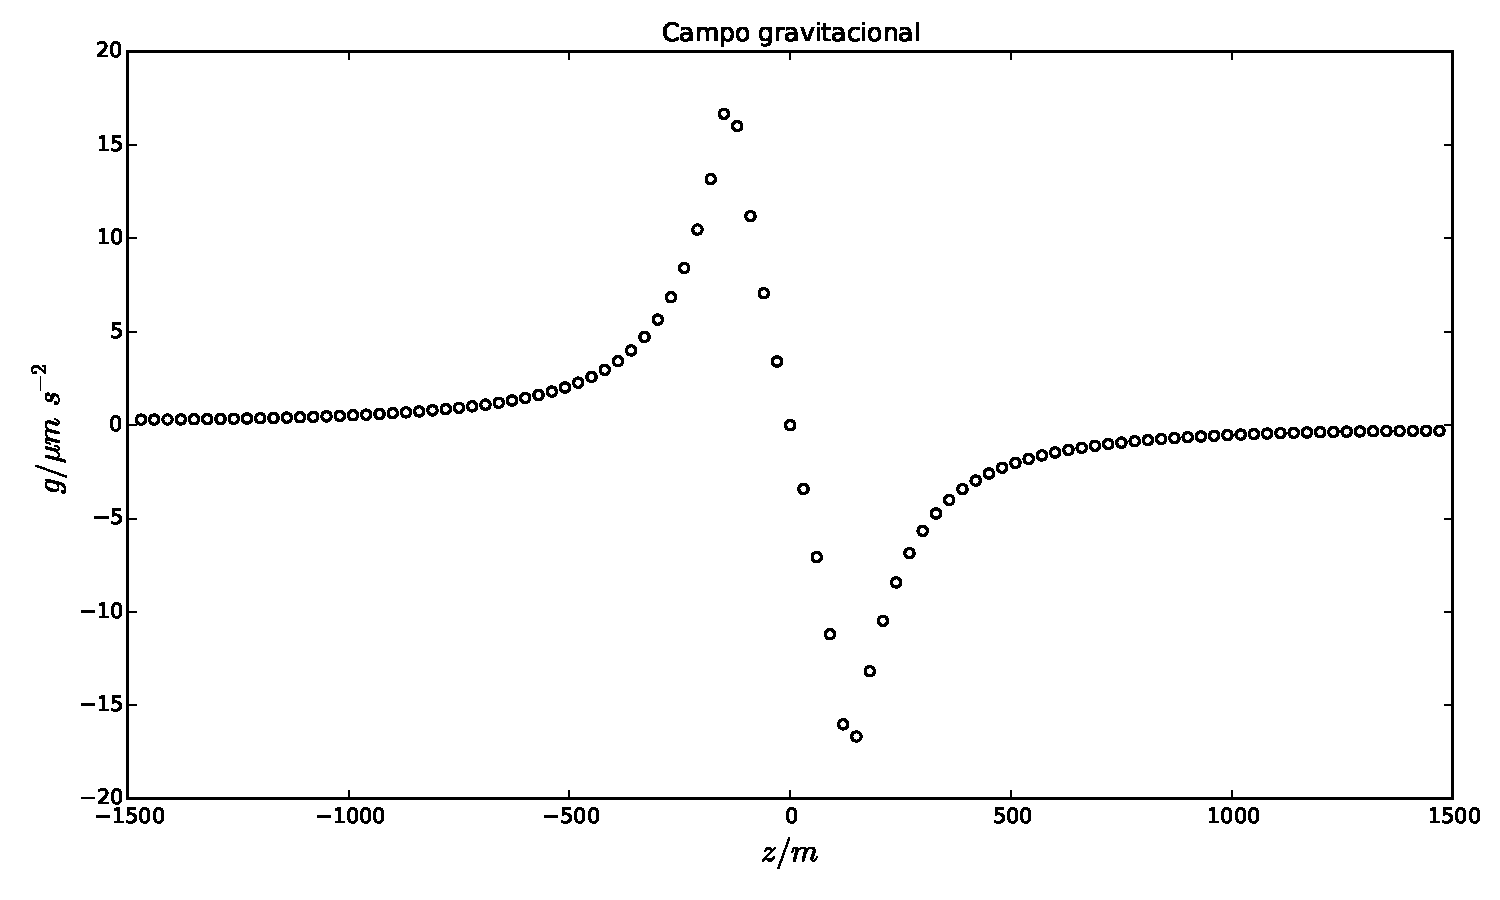
\includegraphics[width=0.85\textwidth]{./accel.pdf}
\end{center}

\part[10] Finalmente encuentre el tiempo que le tomaría a una partícula de masa pequeña en chocar contra el cubo si parte del reposo sobre el eje $z$ y a una distancia de $500\,\textrm{m}$ de la cara más próxima. Para ello resuelva la ecuación de movimiento usando lo encontrado para el campo gravitacional en el anterior literal. 

%Para hacerse a una idea aproximada del tiempo que se está encontrando, demuestre que el tiempo $T$ que demora una partícula que parte del reposo a una distancia $d_i$ de una partícula puntual de masa $M$, en llegar a una distancia $d_f$ de la misma es 

%\[T=\frac{d_i}{\sqrt{2 M G}} * \left( \sqrt{\frac{d_f(d_i-d_f)}{d_i}} + \sqrt{d_i}\cos^{-1}(\sqrt{d_f/d_i}) \right).\]

\end{parts}
\end{questions}



\end{document}
